\section{Kristalle}
%einleitung sollte noch an das ende von der Symmetrie angepasst werden
Unter dem Begriff Kristall sollte sich jeder ein Bild machen können. 
Wir werden uns aber nicht auf sein Äusseres fokussieren, sondern was ihn im Inneren ausmacht.
Die Innereien eines Kristalles sind glücklicherweise relativ einfach definiert.
\begin{definition}[Kristall]
    Ein Kristall besteht aus Atomen, welche sich in einem Muster arrangieren, welches sich in drei Dimensionen periodisch wiederholt.
\end{definition}

\begin{figure}
    \centering
    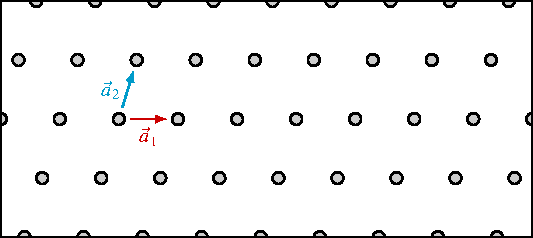
\includegraphics[]{papers/punktgruppen/figures/lattice}
    \caption{
        Zweidimensionales Kristallgitter.
        \texttt{TODO: make wider and shorter}
        \label{fig:punktgruppen:lattice}
    }
\end{figure}
\subsection{Kristallgitter}
Ein zweidimensionales Beispiel eines solchen Muster ist Abbildung \ref{fig:punktgruppen:lattice}.
Für die Überschaubarkeit haben wir ein simples Motiv eines einzelnen grauen Punktes gewählt und betrachten dies nur in Zwei Dimensionen.
Die eingezeichneten Vektoren $\vec{a}$ und $\vec{b}$ sind die kleinstmöglichen Schritte im Raum bis sich das Kristallgitter wiederholt.
Wird ein beliebiger grauer Gitterpunkt in \ref{fig:punktgruppen:lattice} gewählt 
und um eine ganzzahlige Linearkombination von $\vec{a}$ und $\vec{b}$ verschoben, 
endet er zwangsweise auf einem Gitterpunkt, wenn nicht wieder am selben Ort.
Im Dreidimensionalen-Raum können alle Gitterpunkte mit derselben Idee und einem zusätzlichen Vektor $\vec{c}$ also 
\[
    \vec{r} = n_1 \vec{a} + n_2 \vec{b} + n_3 \vec{c}   
\]
erreicht werden sofern $\{n_1,n_2,n_3\} \in \mathbb{Z}$ sind.
Sind die Vektoren  $\vec{a}$ , $\vec{b}$ , $\vec{c}$ gegeben ,
ist ein Kristallgitter eindeutig beschrieben, weswegen sie auch als Grundvektoren bekannt sind.

\subsection{Translationssymmetrie}
Da sich das ganze Kristallgitter wiederholt, wiederholen sich auch dessen Eigenschaften periodisch mit den Grundvektoren.
Sollte man sich auf einem Gitterpunkt in einem Kristall aufhalten, ist es unmöglich zu wissen, auf welchem Gitterpunkt man sich befindet, 
da die Umgebungen aller Punkte Identisch sind. 
Mit anderen worten: Jedes Kristallgitter $ G $ ist \emph{Translationssymmetrisch} in der Translation 
\[
    Q_i(G) = G + \vec{a_i}
\] wobei der Vektor $a_i$ ein Grundvektor sein muss.
Da die Translationssymmetrie beliebig oft mit allen Grundvektoren angewendet werden kann, 
können wir auch sagen, dass alle Verschiebungen um eine Linearkombination 
der Vektoren $\vec{a}$ , $\vec{b}$ und $\vec{c}$ erlaubt sind oder kurz, um $\vec{r}$. 
Verschiebungen um $\vec{r}$ bewirken demnach keine Veränderungen, 
solange wir ein unendlich grosses Kristallgitter verschieben.

\subsection{Limitierte Kristallsymmetrien}
 Die Translationssymmetrie ist wohl keine grosse Überraschung, wenn man die Abbildung \ref{fig:punktgruppen:lattice} betrachtet.
 Was nicht direkt ersichtlich ist, ist das auch wenn die Grundvektoren frei gewählt werden können, 
 können nur Rotationssymmetrische Kristalle bestimmter Rotationswinkel erzeugt werden.

\begin{figure}
    \centering
    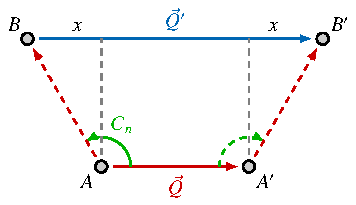
\includegraphics[]{papers/punktgruppen/figures/combine-symmetries}
    \caption{
        Translations und Rotationssymmetrisches Kristallgitter
        \texttt{TODO: make wider and change color (yellow)}
    }
    \label{fig:punktgruppen:rot-geometry}
\end{figure}

 \subsubsection{Translationssymmetrie $Q$ in Kombination mit Rotationssymmetrie $C_\alpha$}     % Müssen uns auf eine schreibweise für Symmetrie Operationen einigen oder sicher am Ende überprüfen
 In Abbildung \ref{fig:punktgruppen:rot-geometry} Sehen wir Gitterpunkte und deren Zusammenhänge.

 \begin{itemize}
     \item  $A$ ist unser erster Gitterpunkt. 

     \item  $A'$ ist gegeben, weil wir $A$ mit der Translation $Q$ um einen Grundvektor verschieben und wir wissen, 
            dass nach einer Translation wieder ein Gitterpunkt an der Verschobenen Stelle sein muss.
     \item $B$ entsteht, weil wir die Rotationssymmetrie $C_\alpha$ auf den Punkt $A$ anwenden.
            Dadurch dreht sich das ganze Gitter um den Winkel $\alpha$. 
            Für uns bedeutet dies lediglich, dass unser zweiter Punkt $A'$ abgedreht wird.
            An der neuen Position von $A'$ muss also auch ein Punkt sein, um die Rotationssymmetrie zu erfüllen.
      \item $B$ ist unser Name für diesen neuen Punkt. 
            Da auch die Eigenschaften des Kristallgittes periodisch mit dem Gitter sein müssen, dürfen wir $C_\alpha$ auch auf $A'$ anwenden.
            Also wenden wir $C_\alpha$ invertiert
            \footnote{Eine Rotationssymmetrie muss auch in die inverse Richtung funktionieren. 
            Genauere Überlegungen hierzu werden dem Leser überlassen, da sich die Autoren nicht explizit mit dieser Frage Auseinander gesetzt haben.} 
            auch auf $A'$ an. 
            Dies dreht $A$ auf einen neuen Punkt.
     \item $B'$ ist kein zufälliger Name für diesen neuen Punkt, denn wir wissen, dass zwischen allen Punkten eine Translationssymmetrie bestehen muss.
            Die Translationssymmetrie zwischen $B$ und $B'$ ist hier als $Q'$ bezeichnet.
 \end{itemize}  
 Mit den gegebenen Punkten lassen sich geometrische Folgerungen ziehen.
 Wir beginnen, indem wir die Länge der Translation $Q$ mit jener von $Q'$ vergleichen.
 Aus Abbildung \ref{fig:punktgruppen:rot-geometry} ist ersichtlich, dass $|Q| = |Q'|+ 2x$.
 Ist $Q$ ein Grundvektor so muss $|Q'|$ ein ganzes vielfaches von $|Q|$ sein. Also 
 \[
    |Q'| = n|Q| = |Q| + 2x
 \]
 Die Strecke $x$ lässt sich auch mit hilfe der Trigonometrie und dem angenommenen Rotationswinkel $\alpha$ ausdrücken:
 \[
    n|Q| = |Q| + 2|Q|\sin(\alpha - \pi/2)
 \]
 Wir können mit $|Q|$ dividieren um unabhängig von der Läge des Grundvektors zu werden, 
 was auch Sinn macht, da eine Skalierung eines Kristalles seine Symmetrieeigenschaften nicht tangieren soll. 
 Zusätzlich können wir den Sinusterm vereinfachen.
 \[
     n = 1 - 2\cos\alpha
     \alpha = \cos^{-1}\left(\frac{1-n}{2}\right)
 \]
 Dies schränkt die möglichen Rotationssymmetrien auf 
 \[
     \alpha \in \left\{ 0^\circ, 60^\circ, 90^\circ, 120^\circ, 180^\circ\right\}
 \]
ein.

\begin{figure}
    \centering
    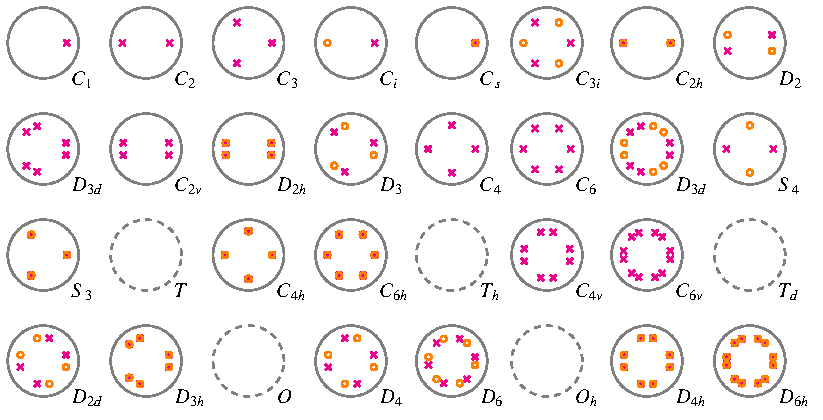
\includegraphics[]{papers/punktgruppen/figures/projections}
    \caption{Kristallklassen mit zugehöriger Schönfliesnotation}
    \label{fig:punktgruppen:Kristallkassen}
\end{figure}

\subsection{Kristallklassen}
Vorgehend wurde gezeigt, dass in einem zweidimensionalen Kristallgitter nicht alle Symmetrien möglich sind.
Mit weiteren ähnlichen überlegungen gezeigt werden kann, dass Kristalle im dreidimensionalen Raum
\footnote{Alle $17$ möglichen zweidimensionalen Symmetrien sind als Wandmustergruppen bekannt} 
nur auf genau $32$ Arten punktsymmetrisch sein können.
Diese $32$ möglichen Punktsymmetrien scheinen durchaus relevant zu sein, denn sie werden unter anderem als Kristallklassen bezeichnet.
Eine mögliche Art, die Klassen zu benennen ist nacht dem Mathematiker Arthur Moritz Schönflies, 
welcher sich mit der Klasifizierung dieser Symmetrien auseinandergesetzt hat.
Auf der Abbildung \ref{fig:punktgruppen:Kristallkassen} sind die möglichen Punktsymmetrien mit deren Schönfliesnotation aufgelistet.
Als Darstellungsmethode wurde die stereographische Projektion gewählt, wobei $5$ Klassen aus Gründen der Überschaubarkeit nicht gezeichnet wurden.  



